\section{Sujet}

\subsection{L'interface}

L'interface d'OpenSCAD est composée de plusieurs fenêtres :


\begin{figure}[ht]
	\centering
	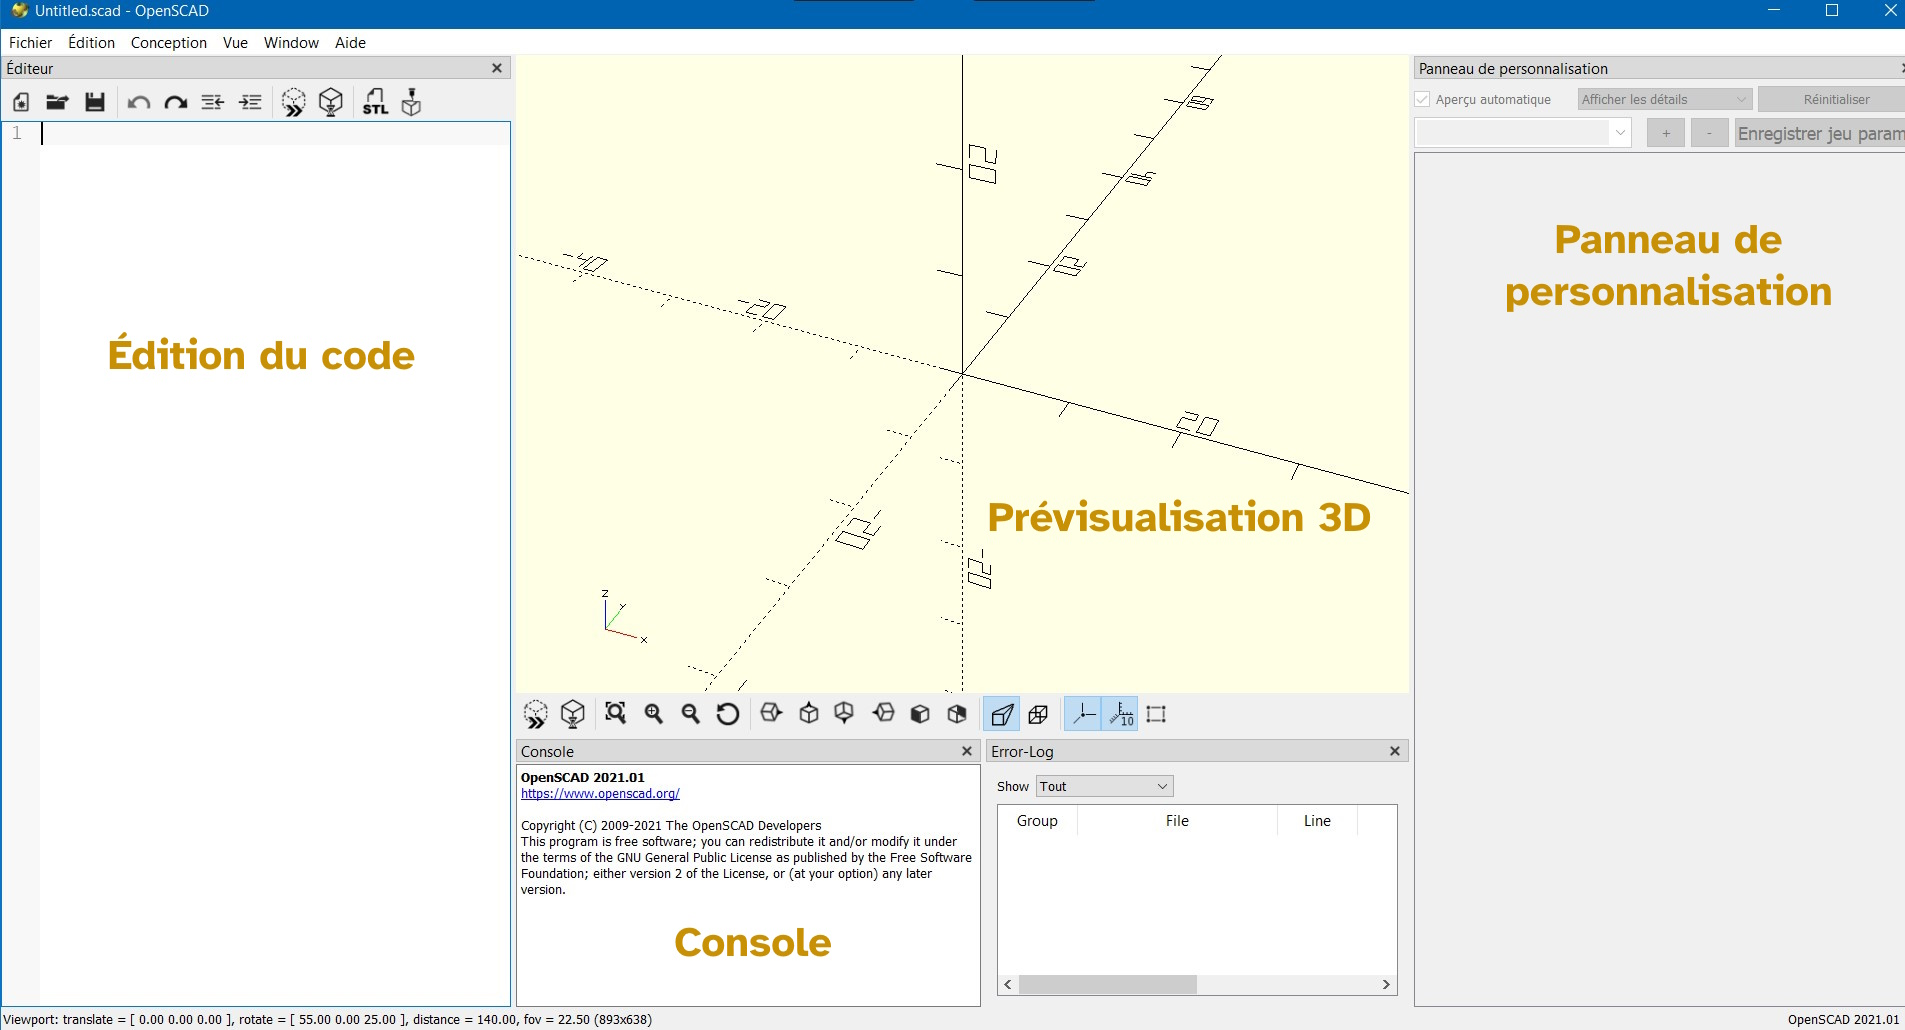
\includegraphics[width=12cm]{images/interface}
	\caption{\textit{Interface d'OpenSCAD}}
\end{figure}


\subsubsection{Éditeur}

C'est dans cette fenêtre que tout le code doit être écrit.
Le fonctionnement est semblable à n'importe quel éditeur classique, il faut rédiger le programme ligne par ligne, elles mêmes numérotées.
L'éditeur d'OpenSCAD fournit un système d'autocomplétion qui peut s'avérer très utile pour connaître rapidement la syntaxe attendue.


\subsubsection{Prévisualisation 3D}

Cette fenêtre permet de visualiser rapidement le rendu 3D décrit par le code.
Il n'est pas possible d'éditer directement les objets dans cette fenêtre.
Toutefois vous pouvez naviguer et explorer le modèle sous tous ses angles, afin de vérifier que le rendu correspond à vos attentes.

Vous pouvez modifier le thème de cette fenêtre en allant dans \textit{édition > préférences > vue 3D}.

Il est également possible de sélectionner les éléments que vous souhaitez voir dans la barre de boutons située au pied de la fenêtre.
Dans cette même barre, des boutons vous permettent de positionner la vue selon des orientations particulières (par exemple parfaitement au dessus du modèle).


\subsubsection{Console}

La console affiche les différentes informations lors de la compilation, le processus de transformation du code vers le modèle 3D.
Elle permet de voir les potentiels avertissements ou erreurs afin de les corriger.


\subsubsection{Panneau de personnalisation}

Nous n'utiliserons pas cette fenêtre dans cet atelier, elle est destinée à des utilisateurs avancés.


\subsection{Premiers pas}

\subsubsection{Formes basiques}

OpenSCAD dispose de plusieurs objets simples pour entamer la création de modèles : 
\verb|square|, \verb|circle|, \verb|cube|, \verb|cylinder| et \verb|sphere|.

Créons par exemple un cube d'1cm de côté. Pour cela il suffit d'écrire \verb|cube(1);| dans l'éditeur.
Ensuite, il faut appuyer sur la touche \verb|F5| de votre clavier pour pouvoir calculer l'aperçu.

\begin{figure}[ht]
	\centering
	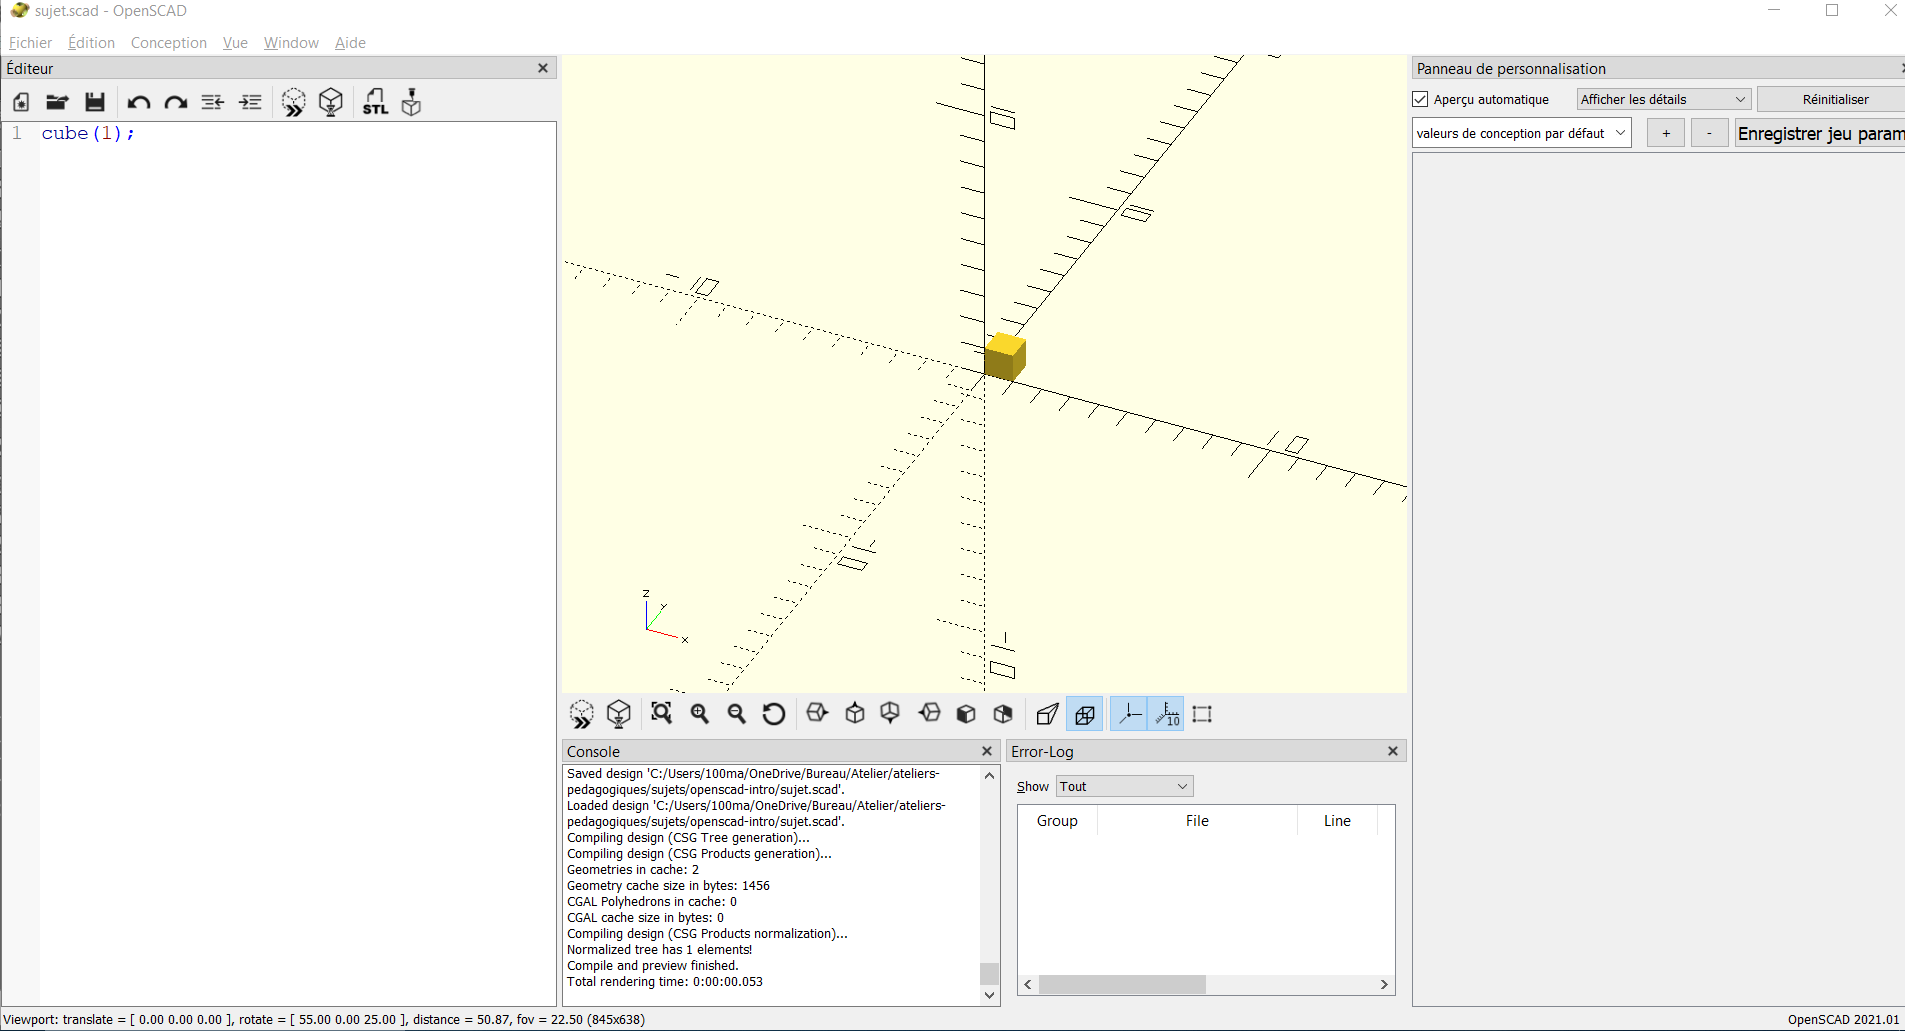
\includegraphics[width=12cm]{images/cube_1}
	\caption{\textit{Simple cube d'1cm de côté}}
\end{figure}

Rajoutons maintenant un pavé de 2cm de long, 2cm de large et 0.5cm de haut.
Cela se fait également avec la \textbf{fonction} \verb|cube| mais cette fois en mettant une liste de valeurs en \textbf{paramètre} : \verb|cube([2,2,0.5]);|.

\begin{figure}[ht]
	\centering
	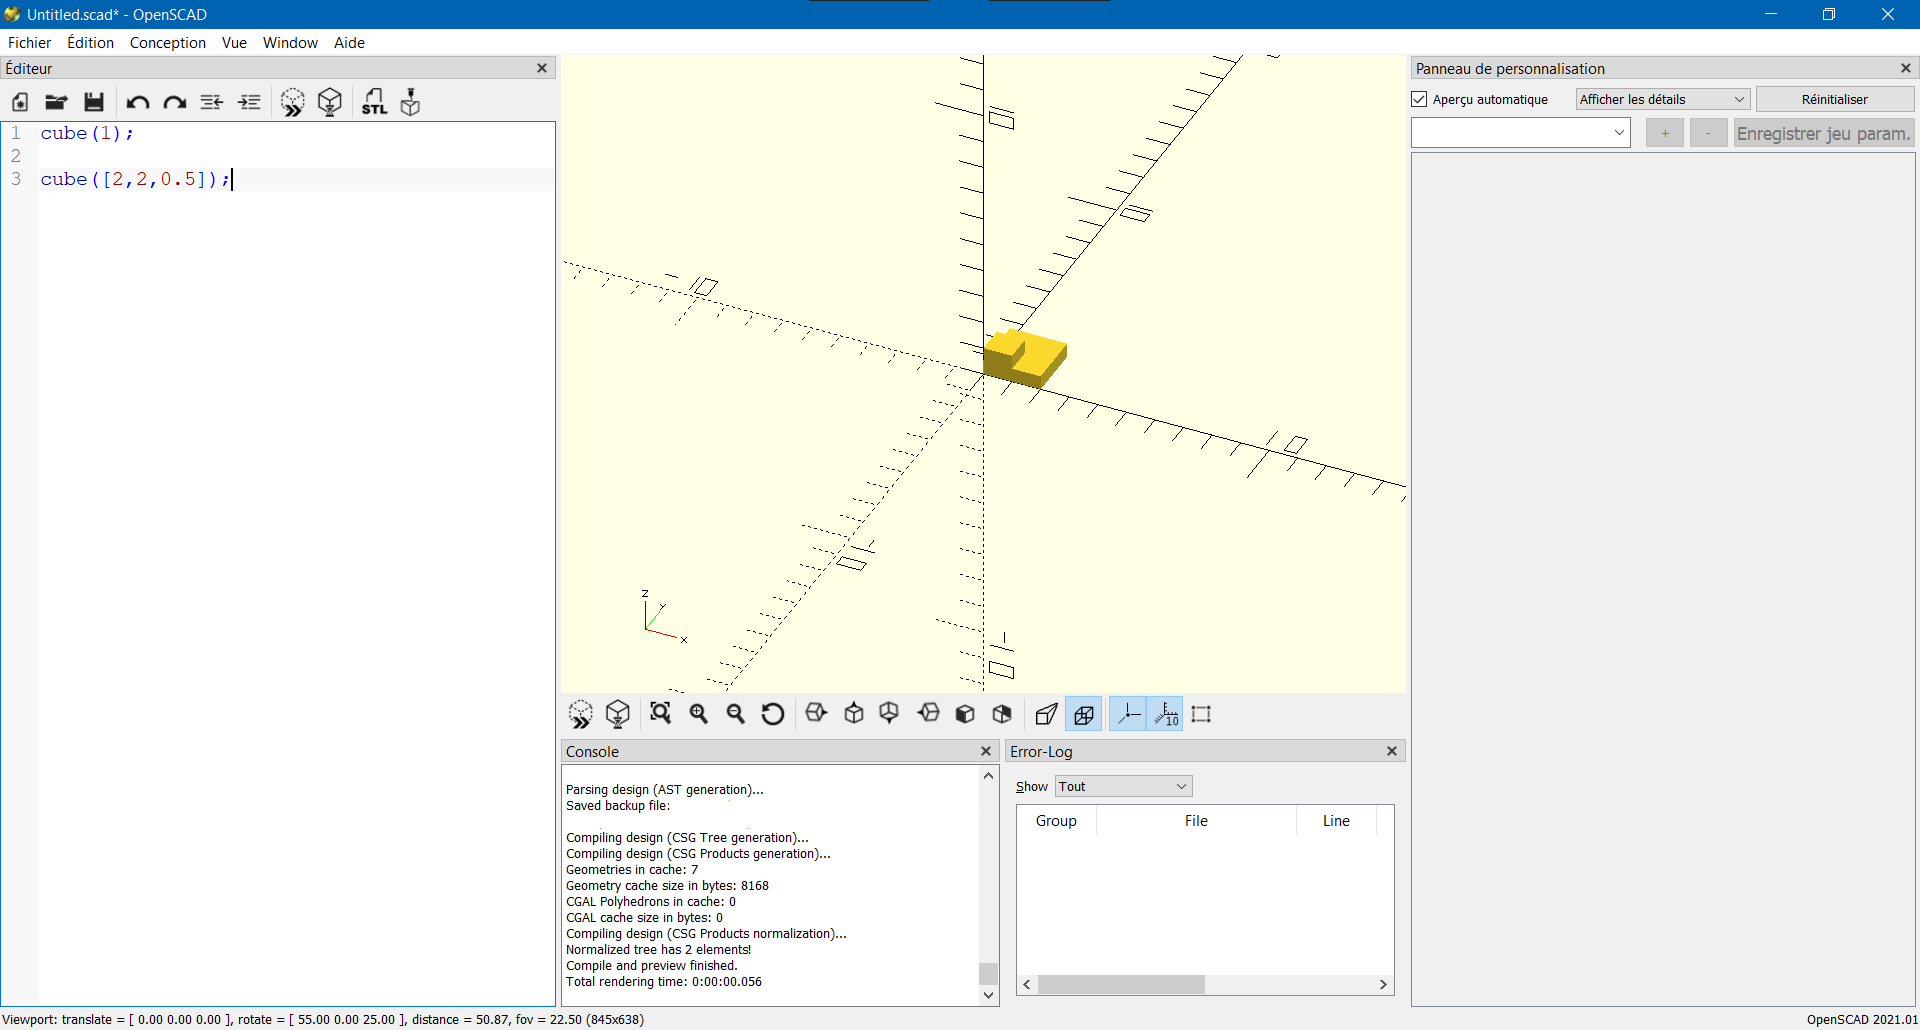
\includegraphics[width=12cm]{images/cube_2-2-05}
	\caption{\textit{Pavé droit}}
\end{figure}